%%%%%%%%%%%%%%%%%%%%%%%%%%%%%%%%%%%%%%%%%%%%%%%%%%%%%%%%%%%%%%%%%%%%%%%%%%%%%%%%
%     Escape rate for a Brownian particle in a radial cubic spline trap        %
%                           Marc Meléndez Schofield                            %
%%%%%%%%%%%%%%%%%%%%%%%%%%%%%%%%%%%%%%%%%%%%%%%%%%%%%%%%%%%%%%%%%%%%%%%%%%%%%%%%

%%%%%%%%%%%%%%%%%%%%%%%%%%%%%%%%%%%% Head %%%%%%%%%%%%%%%%%%%%%%%%%%%%%%%%%%%%%%

\documentclass{article}
\usepackage[utf8]{inputenc}
\usepackage{amsmath}
\usepackage{comment}
\usepackage{graphicx}
\usepackage{listings}

\title{Escape rate for a Brownian particle in a radial cubic spline trap}
\author{Marc Meléndez}

%%%%%%%%%%%%%%%%%%%%%%%%%%%%%%%%%%%% Body %%%%%%%%%%%%%%%%%%%%%%%%%%%%%%%%%%%%%%

\begin{document}

\maketitle

%! codeblock: introduction
Brownian motion has many applications in mathematics, physics and finance, but
it was originally conceived as the description of small micron-scale particles
suspended in water, which vibrate due to thermal fluctuations. Here, we are
interested in a Brownian particle that moves around in two dimensions and feels
the force due to a particular type of potential energy trap. We aim to describe
the time it takes for such a particle to escape from the trap.
%! codeblockend

\section{Cubic spline trap}

Let $r$ represent the distance between the position of a Brownian particle and
the centre of a cubic spline trap, and let $V(r)$ represent the potential energy
of such a particle (see Fig. \ref{cubic_spline}). We choose $V(r)$ in such a way
that the depth of the trap equals $E_0$, its radius is $R$ and, that it lies
flat at the origin and at $r = R$ (so $V'(0) = V'(R) = 0$).
\begin{equation}
  V(r) =
  \begin{cases}
    E_0 \left(-2\left(\frac{r}{R}\right)^3
              + 3 \left(\frac{r}{R}\right)^2 - 1\right), & \text{for } r < R, \\
    0, & \text{for } r \geq R.
  \end{cases}
\end{equation}
A trapped particle, then, feels a force
\begin{equation}
  \mathbf{F}(\mathbf{r}) = -\nabla V
                         = \frac{6}{R^2}
                           \left(\frac{r}{R} - 1\right)\ \frac{\mathbf{r}}{R}.
\end{equation}

\begin{comment}
This gnuplot code produces a graph of $V(r)$, used in the figure below.
%! codefile: cubic_spline.gnuplot
set term postscript eps enhanced size 7cm,4cm font "Roman"
set output "cubic_spline.eps"
set xlabel "{/:Italic r / R}"
set ylabel "{/:Italic V}({/:Italic r/R}) {/:Italic / E}_0"
plot [0:1.5][-1.2:0.2] (x<1)?-2*x**3 + 3*x**2 - 1:0 w l lw 3 lc -1 notitle, \
                       0 w l lc -1 dt 2 notitle
%! codeend
\end{comment}

\begin{figure}
  \centering
  \includegraphics[width=\linewidth]{cubic_spline.eps}
  \caption{\label{cubic_spline}Radially symmetrical cubic spline trap of depth
           $E_0$.}
\end{figure}

We wish to determine the rate at which a trapped Brownian particle escapes from
the trap. Dimensional analysis reveals that the rate $\mu$ equals
\begin{equation}
\label{dimensional_analysis}
  \mu = \frac{D}{R^2}\ f\left(\frac{E_0}{k_BT}\right),
\end{equation}
where $D$ stands for the diffusion coefficient, $k_BT$ the thermal energy, and
$f$ for an as yet undetermined function.

\section{Numerical simulation}

We can check our predictions by setting up a numerical simulation of the process
process. A minimal C program could accept $E_0$, $R$, $D$ and $k_BT$ as
parameters.

\lstset{language = c, morecomment = [is]{\%!}{\^^M}}
\begin{lstlisting}[frame=single]
%! codeblock: usage_message
  /* Usage message */
  if(argc < 5) {
    fprintf(stderr, "Usage: %s <trap depth> "
                              "<trap radius> "
                              "<diffusion coefficient> "
                              "<thermal energy>\n",
            argv[0]);
    return 0;
  }
%! codeblockend
\end{lstlisting}


\begin{comment}
%! codefile: cubic_spline.c
# include <stdio.h>
# include <stdlib.h>
# include <math.h>
# include "random.h"

int main(int argc, char * argv[])
{
  %! codeinsert: usage_message

  %! codeinsert: variable_declarations

  %! codeinsert: Brownian_simulation

  %! codeinsert: output_results

  return 0;
}
%! codeend
\end{comment}

Following the usage message, we declare the values and parameters needed for the
Brownian simulation. The jagged trajectory of Brownian motion results from
integrating the (It\=o) stochastic differential equation
\begin{equation}
  d\mathbf{r} = M \mathbf{F}(\mathbf{r})\ dt + \sqrt{2 D}\ d\mathbf{W},
\end{equation}
where $M = D/k_BT$ stands for the particle mobility, $-\nabla V$ is the force
due to our cubic spline trap and $d\mathbf{W}$ is the two-dimensional Wiener
process.

\begin{lstlisting}[frame=single]
%! codeblock: variable_declarations
  /* Variable declarations */
  int nruns = 10000;    /* Number of runs */
  int run;              /* Current run */
  double q[2];          /* Particle position */
  double F[2], Fmod;    /* Force and modulus of force*/
  double r;             /* Distance to origin */
  long int tstep;       /* Current step */
  long int sumtime = 0; /* Sum of times */
  long int sumt2 = 0;   /* Sum of times squared */

  /* Simulation parameters */
  double E0 = atof(argv[1]); /* Trap depth */
  double R = atof(argv[2]);  /* Trap radius */
  double D = atof(argv[3]);  /* Diffusion coefficient */
  double kT = atof(argv[4]); /* Thermal energy */
  double M = D/kT;           /* Mobility */
  double dt = 0.0001;        /* Time step */
%! codeblockend
\end{lstlisting}

The \texttt{nruns} realisations of the stochastic process proceed by setting the
Brownian particle at the origin of coordinates and then letting it diffuse until
it reaches the edge of the trap at $r = R$. An Euler-Maruyama scheme integrates
the equations of motion. \texttt{Gaussian(0,1)} produces a random number from a
normal distribution with null mean and unit standard deviation.

\begin{lstlisting}[frame=single]
%! codeblock: Brownian_simulation
  /* nruns realisations of the stochastic process */
  for(run = 0; run < nruns; run++) {
    /* Reset position */
    q[0] = q[1] = 0.0;

    /* Run Brownian dynamics until particle escapes */
    for(tstep = 0; 1; tstep++) {
      /* Particle position */
      r = sqrt(q[0]*q[0] + q[1]*q[1]);

      /* Break when particle leaves the trap */
      if(r >= R) break;

      /* Force vector */
      Fmod = 6.0*E0*(r/R - 1)/(R*R*R);
      F[0] = Fmod*q[0];
      F[1] = Fmod*q[1];

      /* Euler-Maruyama scheme */
      q[0] += M*F[0]*dt + Gaussian(0,1)*sqrt(2*D*dt);
      q[1] += M*F[1]*dt + Gaussian(0,1)*sqrt(2*D*dt);
    }

    sumtime += tstep;
    sumt2 += tstep*tstep;
  }
%! codeblockend
\end{lstlisting}

The code ends by outputting the results, calculating the inverse of the mean
time it took the Brownian motion to escape from the trap.

\begin{lstlisting}[frame=single]
%! codeblock: output_results
  float meantime = (sumtime*dt)/((float) nruns);
  float mu = 1.0/meantime;

  printf("# E0 \t\t R \t\t D \t\t kT \t\t "
         "mu \t\t error(mu)\n");
  printf("%f\t%f\t%f\t%f\t%f\t%f\n", E0, R, D, kT, mu,
          mu*mu*sqrt((sumt2*dt*dt)/((float) nruns)
                     - meantime*meantime)/sqrt(nruns));
%! codeblockend
\end{lstlisting}


\section{Numerical results}

The first very obvious test of the code verifies that $\mu$ is indeed
proportional to $D$ and inversely proportional to $R^2$, as stated by Eq.
(\ref{dimensional_analysis}). Fig. \ref{mu_vs_D_and_R} shows that the
simulations agree with this prediction, although smaller values of $R$
depart from the curve, probably due to issues with the integration time
step.

\begin{comment}
With an operating cubic_spline program, we can easily generate the data files
using a bash script.
%! codefile: cubic_spline.sh
#!/bin/bash
for D in `seq 0.2 0.2 2`; do ./cubic_spline 1 1 $D 1; done | grep -v "#" > mu_vs_D.dat
for R in `seq 1 0.2 3`; do ./cubic_spline 1 $R 1 1; done | grep -v "#" > mu_vs_R.dat
for E0 in `seq 0.25 0.25 7.5`; do ./cubic_spline $E0 1 1 1; done | grep -v "#" > mu_vs_E0.dat
%! codeend

The next figure plots $mu$ versus D and R to check the validity of Eq.
(\ref{Dimensional analysis}).

%! codefile: mu_vs_D_and_R.gnuplot
set term postscript eps enhanced size 8cm,4cm font "Roman"
set output "mu_vs_D_and_R.eps"
set ylabel "{/Symbol m} [a.u.]"
set size square

f(x) = a*x
fit f(x) "mu_vs_D.dat" u 3:5 via a
g(x) = b/(x**2)
fit g(x) "mu_vs_R.dat" u 2:5 via b

set multiplot layout 1,2
set xlabel "{/:Italic D} [a.u.]"
plot [0:2][0:6] "mu_vs_D.dat" u 3:5:6 w errorbars notitle lc -1, \
                f(x) w l dt 2 lc -1 notitle
set xlabel "{/:Italic R} [a.u.]"
plot [0:3][0:5] "mu_vs_R.dat" u 2:5:6 w errorbars notitle lc -1, \
                g(x) w l dt 2 lc -1 notitle
unset multiplot
%! codeend
\end{comment}

\begin{figure}
  \centering
  \includegraphics[width=\linewidth]{mu_vs_D_and_R.eps}
  \caption{\label{mu_vs_D_and_R}Escape rate $mu$ versus diffusion coefficient
           $D$ (\textit{left}) and trap radius $R$ (\textit{right}) confirming
           the relation predicted by Eq. (\ref{dimensional_analysis}). The
           dotted lines follow fits with the theoretical tendencies.}
\end{figure}

\section{Theoretical considerations}



% \begin{figure}
%  \centering
%  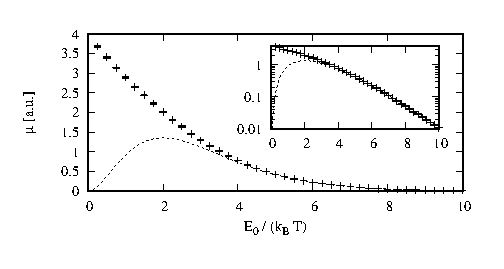
\includegraphics[width=\linewidth]{mu_vs_E0.eps}
%  \caption{\label{mu_vs_E0}...}
% \end{figure}

\end{document}

%%%%%%%%%%%%%%%%%%%%%%%%%%%%%%%%%% Makefile %%%%%%%%%%%%%%%%%%%%%%%%%%%%%%%%%%%%

%! codefile: Makefile
all: tangle code data figures weave

tangle:
	txt2tangle kramers.tex

code:
	gcc -Wall -march=native -Ofast -lm -o cubic_spline cubic_spline.c

data:
	bash cubic_spline.sh

figures:
	gnuplot cubic_spline.gnuplot
	gnuplot mu_vs_D_and_R.gnuplot

weave:
	latex kramers.tex
	dvips kramers.dvi
	ps2pdf kramers.ps
%! codeend

%! codefile: README.md

# Escape rate for a Brownian particle in a radial cubic spline trap

%! codeinsert: introduction

## Aim

This short project illustrates literate programming using the **txt2tangle**
tool. You can check out the final result in the **kramers.pdf** file.

## Compiling and running

This project assumes that your system has the following tools installed:
**txt2tangle**, **make**, **gcc**, **bash**, **gnuplot**, **latex**, **dvips**
and **ps2pdf**. *All* the files for this project (including this one) stem from
**kramers.tex**. By running `txt2tangle kramers.tex`, you can generate the
`Makefile`. Everything else in the project (compiling, running and outputting
the final report) takes place when you execute `make`.

%! codeend
